% MIRU2015: How to use the LaTeX class Ver.1
\documentclass[MIRU]{miru2015e}
\usepackage{graphicx}
\usepackage{latexsym}
%\usepackage[fleqn]{amsmath}
%\usepackage[psamsfonts]{amssymb}

\begin{document}

%\title{Combining High-level Feature Attributes for Semantic Video Classification}
\title{Semantic Video Classification by Fusing Multimodal High-Level Features}

\affiliate{Montreal}{Faculty of Engineering \& Computer Science, Concordia University, Montreal, Canada}
\affiliate{Yokosuka}{Media Intelligence Lab, NTT, 1-1 Hikarinooka, Yokosuka, Kanagawa, 239--0847, Japan}

\author{Olivier Nguyen}{Montreal}[nguyenolive@gmail.com]% 
\author{Yongqing Sun}{Yokosuka}[yongqing.sun@ntt.co.jp]% 
\author{Kyoko Sudo}{Yokosuka}[sudo.kyoko@ntt.co.jp]% 
\author{Akira Kojima}{Yokosuka}[kojima.akira@ntt.co.jp]% 

%Abstract and keywords should be omitted

\maketitle

\section{Introduction}
The rapidly growing video-recording capabilities and enormous amount of user content being generated on the internet everyday demands new, effective methods for automatic recognition and indexing of visual content.

Most studies in past years in the field of image and video recognition have focused mainly on low-level visual features as they have proven to be robust and reliable \cite{liobjectbank}. However, there is still a semantic gap; there is a lack of meaning in the represented data between the feature and the actual video content. In recent years, the study of attributes has attracted much research interest for multimedia analysis where these high-level representations of media carry more substantial information than low-level features. Notably, the Object Bank (OB) representation models an image based on the objects that appear in them \cite{liobjectbank}. An extension of this idea for actions in a video is the Action Bank (AB) method. 

We examine a method that extends these two ideas by combining them using various fusion algorithms to improve the semantic representation for event recognition. We believe that OB and AB complement each other because together they suggest the idea that a video or event is better recognized by the basic objects and actions occurring in it. %Our preliminary experiments demonstrate that our method is comparable to the best performing techniques on data sets like UCF50 and HMDB51 with late fusion of OB and AB using a simple linear SVM classifier.

\section{Investigated Method}

\subsection{Feature Extraction}
\subsubsection{Object Bank}
The OB representation depicts an image as an aggregation of the objects contained in it. The feature vector for OB is derived from object detectors that produce a high-dimension output from 177 object detectors taken at various scales and positions in the original image, which results to 252 responses per detector (44,604 dimensions for a single image) \cite{liobjectbank}. After extracting the key frames, the OB feature vectors were extracted for every image and then max-pooling is applied across all frames to represent the video with a single feature vector.

\subsubsection{Action Bank}
Similarly, AB attempts to be a high-level representation of activity occurring in video. The AB feature vector is the output of many individual template-based action detectors sampled broadly in semantic space and viewpoint space \cite{corsoab}. The output of the 205 action detectors have 73 dimensions each, which are concatenated to form the final action bank representation of 14,965 dimensions. The publicly published AB features were used to conduct the experiments\footnote{www.cse.buffalo.edu/{\raise.17ex\hbox{$\scriptstyle\sim$}}jcorso/r/actionbank/}.

\subsection{Feature Representation}
We performed mean-pooling on the responses of each detector to form one component, leading to a feature vector of size 177 and 205 for OB and AB respectively. The dimensions were reduced so that a feature vector can be viewed as a representation of absence/presence of objects and actions in a video while discarding information about the detector's positions \cite{obdimreduce}.

\subsection{Fusion Methods}
The two common fusion methods were experimented i.e. early fusion and late fusion. Early fusion is a simple way of combining multiple features together before the classification, hence it consists of concatenating multiple features to form a single feature vector. 

Late fusion combines the individual classifiers at the decision level in order to make predictions. Late fusion methods use the probability scores returned by the SVM classifiers (Figure 1). We used a probabilistic method from \cite{latefusion} by combining the posterior class probabilities output by each classifier, which are computed as a weighted sum of the scores for each modality. The weighted averaging (WA) technique is described as:
\[p(c|x_{1}, ..., x_{M}) = \sum\limits_{i=1}^M p(c | x_{i}) \alpha_{i}\]
 where c is the class,  $x_{i}$ is the individual feature,  M is the number of descriptors, and the weights \(\alpha_{i}\) sum to 1 and indicate the reliability of each features. The weights are chosen by optimizing the mean accuracy metric through an exhaustive grid-search.

Logistic regression (LR) is another late fusion method that was explored to convert the M-dimensional vector of scores into a single value to make decisions.

\subsection{Training of Classifiers}

We chose a combination of linear and RBF SVM classifiers for late fusion (Figure 1) with the hyper-parameters and kernel optimized through grid-search and cross-validation. We used an SVM implementation provided by the scikit-learn library\footnote{www.scikit-learn.org/} and a one-vs-all training scheme for multi-class classification, with the input feature vectors scaled between 0 and 1.

To perform decision-level fusion, we train two separate classifiers on each features individually. From the resulting two probability outputs, weighted averaging is computed as described previously. We train a third classifier with the result from the weighted averaging, which produces the final classification and prediction.	

\begin{figure}
\centering
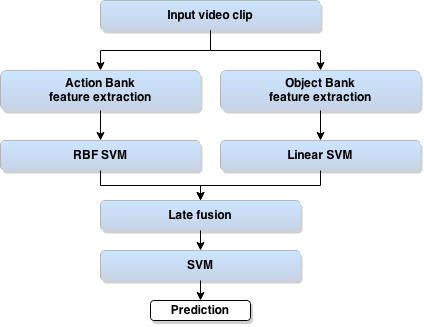
\includegraphics[width=3in]{overview.png}
\caption{High-level System overview}
\label{overview}
\end{figure}

\section{Experiments}

\subsection{Video Dataset}
We chose to use the UCF50 and HMDB51 databases which are common benchmarks for video classification. They both contain a large number of categories, 50 and 51 respectively each consisting of over 100 clips, and they also have unconstrained videos from popular websites like YouTube \cite{hmdb}. Both these data sets are challenging due to their large variations in camera motion, object appearance and cluttered backgrounds \cite{ucf50}. 

\subsection{Evaluation}
Our tests follow the same experimental procedures recommended by the authors of each data set. For UCF50, leave one group out cross-validation \cite{ucf50} was used. As for HMDB51, we used three train-test splits provided by the authors \cite{hmdb}, where each split has 70 training and 30 testing clips for each class. The metric for evaluating the performance of the methods was mean accuracy.

\subsection{Discussion}
It is seen how AB and OB are complementary to each other by observing the late fusion results that yield an accuracy of 68.7\% (Table 1) for UCF50 using weighted average, which is a notable difference of over +10.0\% on top of each individual features. 

However, our method performs poorly in contrast to the state-of-the art method of improved trajectories \cite{wang}, which has 91.2\% accuracy on the same dataset. The significant difference between our method and the state-of-the-art could be explained by the fact that the individual object detectors used in Object Bank have poor precision (30\% at most) \cite{obdimreduce}. With the object detectors becoming more robust and accurate in the future, there is potential for our method to obtain more significant results. Moreover, the use of additional detectors (more than 200 concepts) for both objects and actions may result in better performance, as suggested by \cite{recommendation}.

\begin{table}[h]
\centering
\caption{Mean accuracy results of our methods}
\begin{tabular}{|ll|ll|}
\hline
\multicolumn{2}{|c|}{HMDB51} & \multicolumn{2}{c|}{UCF50}  \\ \hline
Action Bank          & 25.8\%          & Action Bank         & 55.5\%          \\
Object Bank          & 26.8\%          & Object Bank         & 55.1\%          \\ \hline
\textbf{AB+OB (WA)}  & \textbf{34.2\%} & \textbf{AB+OB (WA)} & \textbf{68.7\%} \\
\textbf{AB+OB (LR)}  & \textbf{33.3\%} & \textbf{AB+OB (LR)} & \textbf{67.4\%} \\ \hline
\end{tabular}
\end{table}

\section{Conclusion}
We investigated a simple method with more semantics for video classification through the late fusion of Object Bank and Action Bank which represents a video by objects and actions occurring in it. We hope to further extend the idea by combining our work with that of \cite{wang}, which shows promising results given the success of improved trajectories.
% * <nguyenolive@gmail.com> 2015-05-27T01:51:44.942Z:
%
%  What is meant by "more semantics"
%

\bibliography{references}
\bibliographystyle{ieeetr}

\end{document}